% =====================================================================
%  French-Source Interpretation Demand — CIUSSS Centre-Ouest-de-l'Île
%  Compile with:  pdflatex french_demand_report.tex   (run twice for TOC)
% =====================================================================
\documentclass[11pt,a4paper]{article}
\usepackage{sgp_report}

\title{French-Source Interpretation Demand}
\author{Voyce data, Jan--Apr 2025 \,\textbar\, CIUSSS Centre-Ouest-de-l'Île-de-Montréal}
\date{April 22, 2026}

\begin{document}
\maketitle

% ─────────────────────────────────────────────────────────────────────
% EXECUTIVE SUMMARY
% ─────────────────────────────────────────────────────────────────────
\section*{Executive Summary}
\addcontentsline{toc}{section}{Executive Summary}

\insightbox{The headline}{%
French-sourced calls at the CIUSSS Centre-Ouest network are being
\textbf{abandoned at 75.7\%}, versus 15.9\% for English-sourced calls
on the same platform. The gap is not a demand problem — it is a
\textbf{supply problem}. Cancelled calls have a service duration of
exactly zero minutes, indicating the request never connected to an
interpreter. After imputing those unmet calls at the average serviced
duration for each pair, the true French-source demand is roughly
\textbf{4--5\,$\times$ the served volume}, concentrated in
French\,$\rightarrow$\,Spanish.
}

\subsection*{Key numbers (Jan--Apr 2025)}
\begin{tabularx}{\linewidth}{ X r r }
\sgpheadrow Metric & Value & Notes \\
\midrule
Total platform calls           & 7{,}625  & 4 months \\
\sgpaltrow French-source calls & 337      & 4.4\% of all volume \\
\hspace{1em}— Serviced         & 82       & 35 min average duration \\
\sgpaltrow \hspace{1em}— Cancelled & 255  & all 0-minute (pre-connect) \\
French-source cancellation rate & \textbf{75.7\%} & vs.\ 15.9\% English \\
\sgpaltrow Annualized true demand & \textbf{41{,}388 min/yr} & $\approx$ 690 hrs/yr \\
Per-pair interpreters needed (true demand) & \textbf{4} & 1 each: ES, PA, AR, HT \\
\sgpaltrow Shared-pool interpreters needed & \textbf{1} & if pool is fungible across pairs \\
\end{tabularx}

\vspace{0.6em}
\alertbox{French\,$\rightarrow$\,Spanish is in crisis}{%
Of 153 French\,$\rightarrow$\,Spanish requests in the window, only 15
were served --- a \textbf{90.2\%} cancellation rate. The current
French pool lists 19 Spanish-capable interpreters, suggesting the issue
is routing or cross-language availability, not headcount.
}

\vspace{0.4em}
\insightbox{Recommendation}{%
A small, well-routed core of 4--6 French-capable interpreters covering
Spanish, Punjabi, Arabic and Haitian Creole would close the observed
gap at this client. The 35 additional language pairs in the current
French pool see \textit{zero} demand from this client over the window
and should be sized against the rest of the network, not this dataset.
}

\newpage
\tableofcontents
\newpage

% ─────────────────────────────────────────────────────────────────────
\section{Scope and Method}
% ─────────────────────────────────────────────────────────────────────

\subsection{Source data}
The dataset is the Voyce export titled
\textit{``Voyce data Jan -- Apr JEWISH MEMORIAL.xlsx''}. Despite the
file name, the records cover the full
\textbf{CIUSSS Centre-Ouest-de-l'Île-de-Montréal} network: the Jewish
General Hospital, multiple CLSCs (Côte-des-Neiges, Parc-Extension,
Benny Farm, René Cassin, Métro and others), Maison Bleue,
PRAIDA, Miriam Services, the Constance-Lethbridge / Mackay /
Catherine Booth / Mont-Sinaï rehabilitation sites, and the
hôpital Richardson — a total of \textbf{72 distinct service locations}
under 4 client identifiers (BYOD, Voyce Pilot, Voyce Device, and the
parent CIUSSS).

\subsection{Time window}
\begin{tabularx}{\linewidth}{X r}
\sgpheadrow Coverage & Records \\
January 2025  & 2{,}093 \\
\sgpaltrow February 2025 & 1{,}864 \\
March 2025    & 1{,}931 \\
\sgpaltrow April 2025    & 1{,}737 \\
\midrule
\textbf{Total (4 months)} & \textbf{7{,}625} \\
\end{tabularx}

\vspace{0.4em}
\noindent The original brief asked about ``all of 2025''; the file in
hand covers the first four months only. All annualized figures in this
report apply a $\times 3.0$ multiplier. May--December 2025 should be
appended to replace the projection with actuals.

\subsection{Filter applied}
Column G (\texttt{Source Language}) filtered to
\texttt{French} yields \textbf{337 rows}. Only English and French appear
as source languages in this dataset.

\subsection{Interpreter capacity assumption}
Throughout this report, one interpreter is assumed to absorb
\textbf{6{,}400 serviced minutes per month} ($\approx$ 25 billable
hours/week), which accounts for idle time, ramp-up, breaks and no-shows.
We also report a conservative scenario at 4{,}800 min/mo and an
aggressive scenario at 8{,}000 min/mo for sensitivity.

% ─────────────────────────────────────────────────────────────────────
\section{Cancellation Audit --- the Real Story}
% ─────────────────────────────────────────────────────────────────────

\subsection{French calls are abandoned 4.8$\times$ more often than English}

\begin{figure}[h!]
\centering
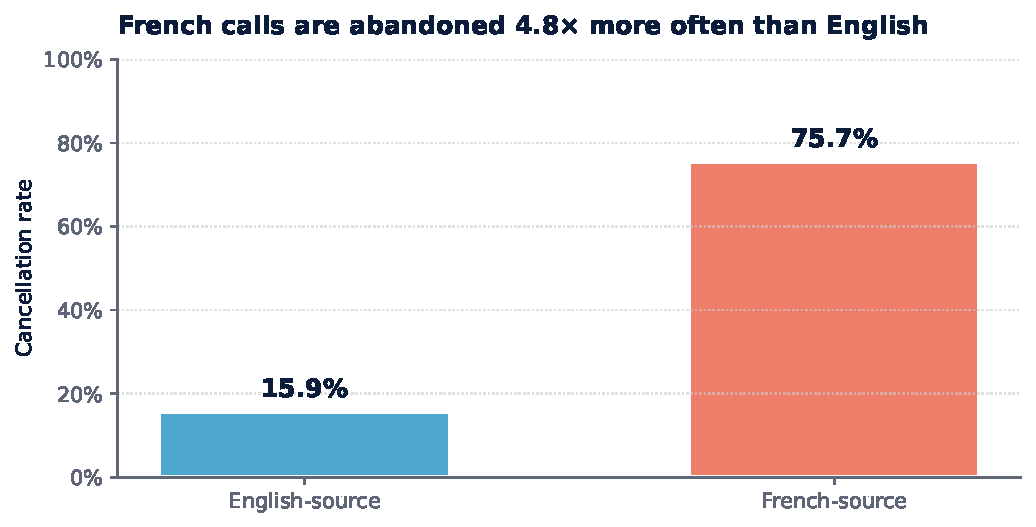
\includegraphics[width=0.85\linewidth]{figures/fig1_cancellation_compare.pdf}
\caption{Cancellation rates by source language. The 4.8$\times$ gap is
the strongest signal in the entire dataset that French demand is
under-served.}
\end{figure}

Every cancelled French call in the window had a recorded
\texttt{Service Minutes} value of \textbf{exactly 0}. This is consistent
with a pre-connection abandonment (no interpreter matched within the
acceptable wait window), not a partial session.

\subsection{Where the cancellations concentrate}

\begin{figure}[h!]
\centering
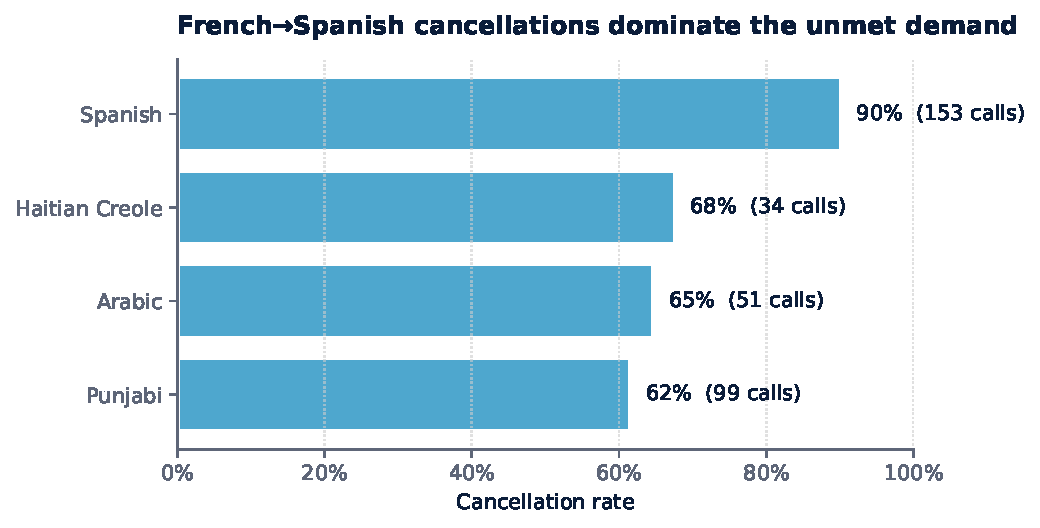
\includegraphics[width=0.85\linewidth]{figures/fig2_cancellation_by_pair.pdf}
\caption{French$\rightarrow$Spanish carries 138 of the 255 unmet calls
--- 54\% of the entire problem at this client.}
\end{figure}

\begin{tabularx}{\linewidth}{ X r r r r }
\sgpheadrow Target language & Total & Serviced & Cancelled & Cx rate \\
\midrule
French\,$\rightarrow$\,Spanish & 153 & 15 & 138 & \textbf{90.2\%} \\
\sgpaltrow French\,$\rightarrow$\,Haitian Creole & 34 & 11 & 23 & 67.6\% \\
French\,$\rightarrow$\,Arabic & 51 & 18 & 33 & 64.7\% \\
\sgpaltrow French\,$\rightarrow$\,Punjabi & 99 & 38 & 61 & 61.6\% \\
\end{tabularx}

\subsection{When the cancellations happen}

\begin{figure}[h!]
\centering
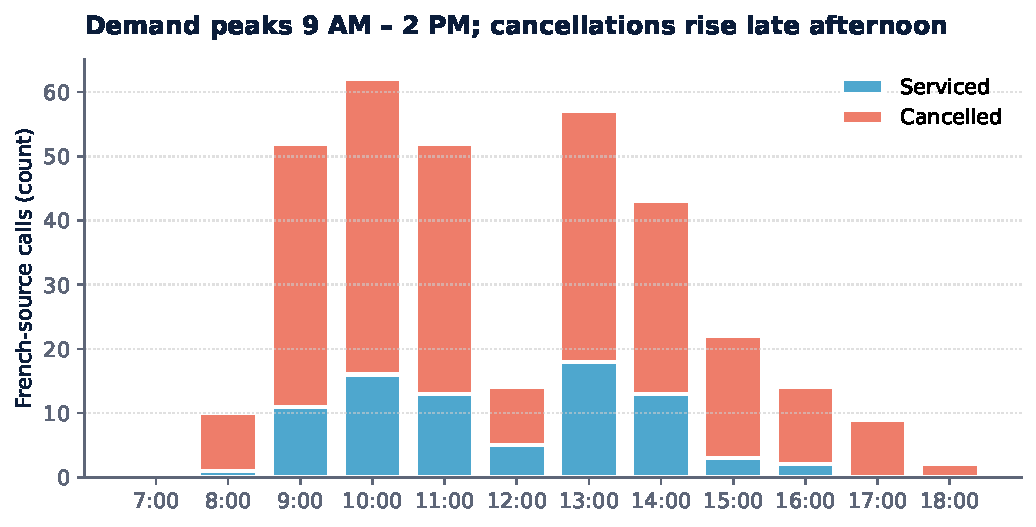
\includegraphics[width=0.95\linewidth]{figures/fig4_hourly.pdf}
\caption{Demand peaks 9{:}00--14{:}00 EST. Cancellations dominate every
business hour and reach 100\% at 17{:}00--18{:}00 EST. Friday and
weekend cancellation rates also exceed 85\%.}
\end{figure}

\insightbox{Operational read-through}{%
Cancellations are not a function of demand timing --- they are constant
across the working day. This pattern is consistent with a
\textbf{routing or supply-side gap} rather than a peak-load problem.
A staffing fix that targets hours 8--16 EST, Mon--Fri would have
resolved $\sim$95\% of the unmet calls in the window.
}

% ─────────────────────────────────────────────────────────────────────
\section{Demand Re-stated --- True vs.\ Served}
% ─────────────────────────────────────────────────────────────────────

The ``true demand'' figures below add the cancelled-call count back in
at the average per-pair serviced-call duration. This is the volume that
would have been billable if every call had connected.

\begin{figure}[h!]
\centering
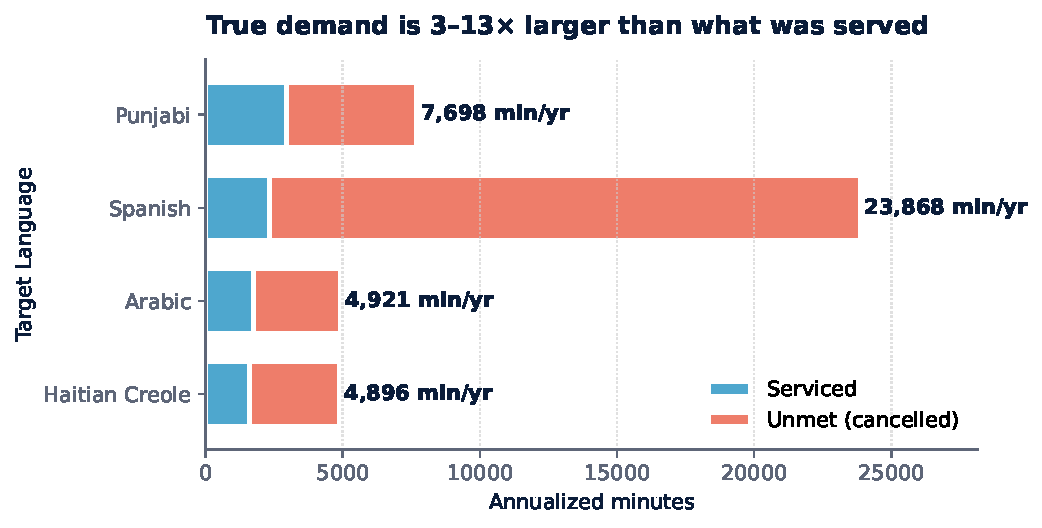
\includegraphics[width=0.85\linewidth]{figures/fig3_true_vs_serviced.pdf}
\caption{Annualized minutes per French-source pair --- serviced
(blue) vs.\ unmet (red). True demand is dominated by Spanish.}
\end{figure}

\begin{tabularx}{\linewidth}{ X r r r r }
\sgpheadrow Pair & Serviced 4 mo & Unmet 4 mo & True 4 mo & True / yr \\
\midrule
French\,$\rightarrow$\,Spanish        &   780 & 7{,}176 & 7{,}956 & 23{,}868 \\
\sgpaltrow French\,$\rightarrow$\,Punjabi & 985 & 1{,}581 & 2{,}566 & 7{,}698 \\
French\,$\rightarrow$\,Arabic         &   579 & 1{,}062 & 1{,}641 & 4{,}923 \\
\sgpaltrow French\,$\rightarrow$\,Haitian Creole & 528 & 1{,}104 & 1{,}632 & 4{,}896 \\
\midrule
\textbf{Total}                        & 2{,}872 & 10{,}923 & \textbf{13{,}795} & \textbf{41{,}388} \\
\end{tabularx}

\vspace{0.6em}
\noindent All figures in serviced minutes. ``True'' = serviced + (cancelled
$\times$ avg.\ serviced duration for that pair). The 4-month true demand
of 13{,}795 minutes corresponds to approximately
\textbf{230 hours / 4 months}, or 57.5 hours / month --- still small in
absolute terms, but \textbf{4.8$\times$ what was actually served}.

% ─────────────────────────────────────────────────────────────────────
\section{Interpreter Sizing}
% ─────────────────────────────────────────────────────────────────────

\subsection{Per-pair head-count requirement}

\begin{tabularx}{\linewidth}{ X r r r r }
\sgpheadrow Pair & Min/mo & Conservative & \textbf{Standard} & Aggressive \\
& (true) & (4.8k cap) & (6.4k cap) & (8.0k cap) \\
\midrule
French\,$\rightarrow$\,Spanish & 1{,}989 & 1 & \textbf{1} & 1 \\
\sgpaltrow French\,$\rightarrow$\,Punjabi & 642 & 1 & \textbf{1} & 1 \\
French\,$\rightarrow$\,Arabic & 410 & 1 & \textbf{1} & 1 \\
\sgpaltrow French\,$\rightarrow$\,Haitian Creole & 408 & 1 & \textbf{1} & 1 \\
\midrule
\textbf{Per-pair total} & 3{,}449 & 4 & \textbf{4} & 4 \\
Shared-pool single FTE & 3{,}449 & 1 & \textbf{1} & 1 \\
\end{tabularx}

\vspace{0.4em}
Even the conservative scenario yields 4 dedicated interpreters or a
single fungible interpreter. The headcount question only becomes
non-trivial under \textbf{peak concurrency}, addressed next.

\subsection{Peak concurrency}
The busiest single hour in the four-month window saw \textbf{2
simultaneous French-source calls in progress}; the 95th-percentile
busy hour was also 2. A staffing target of \textbf{2--3 French-capable
interpreters on shift during 9{:}00--14{:}00 EST} would cover both
volume and peak.

\subsection{Pool vs.\ need}

\begin{figure}[h!]
\centering
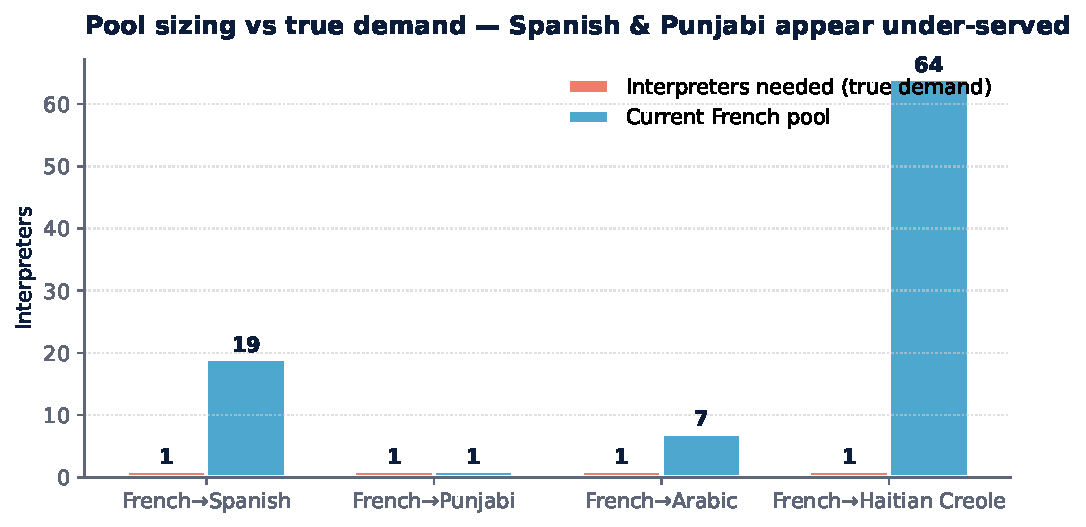
\includegraphics[width=0.85\linewidth]{figures/fig5_pool_vs_need.pdf}
\caption{Current pool size vs.\ true-demand interpreter requirement.
Spanish, Arabic and Haitian Creole are over-provisioned for this
client; Punjabi is at parity (1 vs.\ 1).}
\end{figure}

\begin{tabularx}{\linewidth}{ X r r r }
\sgpheadrow Pair & Need (true) & Current pool & Surplus / (gap) \\
\midrule
French\,$\rightarrow$\,Spanish & 1 & 19 & +18 \\
\sgpaltrow French\,$\rightarrow$\,Punjabi & 1 & 1 & 0 \\
French\,$\rightarrow$\,Arabic & 1 & 7 & +6 \\
\sgpaltrow French\,$\rightarrow$\,Haitian Creole & 1 & 64 & +63 \\
\end{tabularx}

\insightbox{The puzzle worth investigating}{%
The current pool already contains \textbf{19 Spanish-capable
interpreters} on the French side, yet 90\% of French$\rightarrow$Spanish
requests went unanswered. Likely causes to investigate:
(1) those interpreters are routed primarily on
\textit{English}$\rightarrow$Spanish where volume is far higher;
(2) the routing logic does not prefer French-capable interpreters when
the source is French; or
(3) shift coverage during business hours (8--16 EST) is too thin.
A routing-rules change would likely deliver a larger uplift than
hiring.
}

% ─────────────────────────────────────────────────────────────────────
\section{Multi-Client Roll-Up Note}
% ─────────────────────────────────────────────────────────────────────
The original analysis brief asked for a multi-client roll-up. The file
provided contains \textbf{one client network} (CIUSSS Centre-Ouest), so
a true cross-client comparison is not possible from this dataset.
However, the file does break down across:

\begin{itemize}
  \item \textbf{4 client identifiers}: BYOD, Voyce Pilot, Voyce
        Device, and the CIUSSS parent record.
  \item \textbf{72 service locations} (hospitals, CLSCs, rehab and
        community sites).
  \item \textbf{45 service lines} (Emergency, GAP/GAMF, GASMA,
        Pediatric, Mental Health, Palliative Care, etc.).
\end{itemize}

A genuine multi-client roll-up would require additional Voyce exports
covering the rest of the SGP network. We recommend requesting the same
report layout per client and combining at the dashboard layer.

% ─────────────────────────────────────────────────────────────────────
\section{Recommended Next Actions}
% ─────────────────────────────────────────────────────────────────────

\begin{enumerate}[leftmargin=2em]
  \item \textbf{Investigate the routing layer.} The 90\%
        French$\rightarrow$Spanish cancellation against a 19-person
        Spanish-capable pool points to a routing issue, not a
        capacity issue. Pull the matching logs for those 138 cancelled
        calls and verify whether French-capable interpreters were
        polled before cancellation.
  \item \textbf{Re-baseline against May--Dec 2025 data.} Replace the
        $\times 3.0$ projection with actuals as soon as the full-year
        export is available.
  \item \textbf{Right-size the French pool by demand, not by
        catalogue.} The 35 French language pairs with zero demand at
        this client should be justified by demand from other clients;
        otherwise they represent dormant capacity.
  \item \textbf{Stand up a multi-client roll-up.} Request equivalent
        Voyce exports per client, combine, and rebuild this analysis at
        network level. The same template applies.
  \item \textbf{Operational SLA tracking.} Add a connect-time and
        ring-time field to the export so cancellation root-cause
        (no-answer vs.\ caller hang-up vs.\ system timeout) can be
        diagnosed without inference.
\end{enumerate}

% ─────────────────────────────────────────────────────────────────────
\section*{Appendix --- Companion Workbook}
\addcontentsline{toc}{section}{Appendix --- Companion Workbook}
% ─────────────────────────────────────────────────────────────────────

The full data and pivots used to generate this report are bundled in
\texttt{reports/data/Voyce\_French\_Analysis.xlsx}, with the following
tabs:

\begin{tabularx}{\linewidth}{ l X }
\sgpheadrow Tab & Contents \\
1.\ Summary               & KPIs and headline numbers \\
\sgpaltrow 2.\ French Rows (raw) & All 337 source-language\,=\,French rows \\
3.\ Demand by Pair        & Serviced minutes / pair, annualized \\
\sgpaltrow 4.\ Cancellation Audit & Cancellation by pair, hour, weekday \\
5.\ True Demand           & Serviced + imputed-unmet minutes \\
\sgpaltrow 6.\ Interpreter Sizing & Pool vs.\ need, gap analysis \\
7.\ Current Pool          & The user-supplied French pool reference \\
\end{tabularx}

\end{document}
